\documentclass[14pt, letterpaper]{article}
\usepackage[colorlinks=true,linkcolor=black,citecolor=blue,filecolor=cyan,pagecolor=blue]{hyperref} 
\usepackage[toc,style=altlistgroup,hyperfirst=false]{glossaries}
\usepackage[utf8]{inputenc} %para poder escribir símbolos no anglosajones 
\usepackage[spanish, mexico]{babel} %Escribir en español (acentos)
\usepackage[T1]{fontenc}
\usepackage{amssymb}
\usepackage{mathtools}
\usepackage[usenames]{color}
\usepackage{float}
\usepackage{graphicx}  %%para las imagenes
\usepackage{cite} % para contraer referencias
\usepackage{multicol}
\usepackage{multirow}
\usepackage{bm}
\usepackage{bbm}
\usepackage[left=2.5cm,top=2.5cm,right=2.5cm,bottom=2.5cm]{geometry}
\parindent=5mm
\graphicspath{{images/}}
\usepackage{etoolbox}
\let\bbordermatrix\bordermatrix
\patchcmd{\bbordermatrix}{8.75}{4.75}{}{}
\patchcmd{\bbordermatrix}{\left(}{\left[}{}{}
\patchcmd{\bbordermatrix}{\right)}{\right]}{}{}
%%%%glosario
\makeindex
%\makeglossaries
%\input{./glosario.tex}

%%%%%%%%%%%%%%%%%%%%%%%%%%%%%%%%%%%%%%%%%%%%%%%%%%%%%%%%%%%%%%%%%%%%%%%%%%%%%
%%NOTA IMPORTANTE:
%%Para relacionar el glosario.tex con este archivo
%%Es necesario abrir la terminal (Simbolo del sistema en windows)
%%Ir a la carpeta contenedora y escribir el siguiente comando:
%%makeindex -s PROYECTO_final.ist -t PROYECTO_final.glg -o PROYECTO_final.gls PROYECTO_final.glo
%%%%%%%%%%%%%%%%%%%%%%%%%%%%%%%%%%%%%%%%%%%%%%%%%%%%%%%%%%%%%%%%%%%%%%%%%%%%%

%%%% inicio del documento
\begin{document}

\thispagestyle{empty}

%%%%%%% portada

\thispagestyle{empty}

\begin{minipage}[c][0.1\textheight][c]{0.2\textwidth}
\begin{center}
    \includegraphics[width=4cm, height=4cm]{cimat}
\end{center}
\end{minipage}
\begin{minipage}[c][0.1\textheight][t]{0.8\textwidth}
\begin{center}
    {\hspace{2cm}\scshape Centro de Investigación en Matemáticas}
    \vspace{-.5cm}
\end{center}
\hspace*{1.0cm} \rule[0mm]{0.9\textwidth}{0.8mm}
\hspace*{1.17cm}   \rule[4mm]{0.9\textwidth}{0.1mm}
    \vspace{-1cm}
\begin{center}
    { \hspace{2cm}\scshape  Unidad Monterrey}
\end{center}
\end{minipage}

\begin{minipage}[c][0.6\textheight][t]{0.2\textwidth}
\begin{center}
\hskip2pt
\vrule width2.5pt height10cm
        \hskip1mm
        \vrule width1pt height10cm \\ \vspace{2cm}
        \includegraphics[height=4.5cm]{mty}
        \end{center}
\end{minipage}
\begin{minipage}[c][0.9\textheight][t]{0.65\textwidth}
  \begin{center}

	
    \vspace{3.2cm}
    
%%%% TITULO EN PORTADA

  \scshape Proyecto No. 1.\\ \normalsize
  
  \vspace{2cm}  
  
    
            
    Análisis Numérico y Optimización\\
    \vspace{1cm}   
    Algrotimo Kruskal aplicado a rutas de la República Mexicana\\
    \vspace{1cm}   
    \vspace{1cm}   
    Ricardo Cruz Sánchez\\
    \vspace{.5cm}   
  \end{center}
  
\end{minipage}

%TABLA DE INDICES
\pagebreak
\tableofcontents

\cleardoublepage
%INTRODUCCIÓN
\pagebreak
\section{Introducción.}
Un problema que surge de manera natural al considerar el transporte de elementos de interés de un punto a otro es calcular el costo que la operación genera, ya que, esta se busca minimizar.\\

En muchas ocasiones el transporte involucra distintos destinos que se espera visitar y plantear la ruta en la que el costo se minimice no es una tarea trivial.\\

Afortunadamente, se han desarrollado distintos algoritmos con los cuales se puede calcular las rutas en las que el costo se minimiza.\\

Para este trabajo, se considerará que se desea visitar las capitales de los 32 estados de la República Mexicana, tarea que puede ser considerada para una campaña política, transporte de mercancías o simplemente algún viaje que se desee realizar.\\

Los datos, códigos y reportes generados por este proyecto se almacenan en el siguiente repositorio:
\url{https://github.com/Ricardo27cruz27/Algoritmo-Kruskal}


\section{Datos.}

Para calcular la ruta, primero se planteo obtener la representación de las capitales y sus conexiones por carretera a través de un grafo.\\

Primero se obtuvieron las coordenadas de todas las capitales de México. Posterior a esto, con la ayuda de google maps, se calcularon las distancias entre una capital y otra. Tomando como criterio de adyacencia que exisitiera una carretera óptima entre dos capitales sin pasar por otra capital.\\

Por último, con ayuda del aplicativo de la Secretaría de Caminos y transportes, se obtuvieron los costos de casetas para las capitales adyacentes. \\

Con esta información cada nodo adyacente lo conectará una arista con peso equivalente al costo total de casetas y gasolina. La figura 1 muestra el grafo generado.

\begin{figure}
\centering
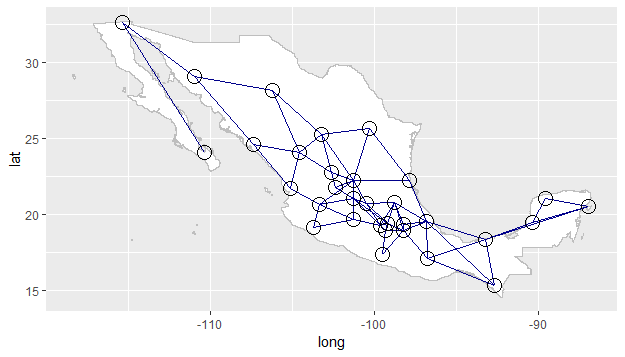
\includegraphics[scale=1]{i1.png} 
\label{i1}
\caption{Grafo generado para las capitales.}
\end{figure}


\section{Aplicativo}
Para calcular el costo hacen falta dos variables para modelar, la primera de ellas, es el precio de la gasolina al momento de ejecutar el modelo, la segunda es el rendimiento kilometros por litro de gasolina del automovil en el que se transportará. Así, el costo generado por la gasolina para cada par de nodos adyacentes se calcula como: el precio del litro de gasolina, por la distancia entre las dos capitales entre el rendimiento por litro.\\

Como este par de variables no son estaticas en el tiempo, se generó un aplicativo en el cual el usuario pueda ingresar manualmente el valor de dichas variables y así poder ejecutar el algoritmo Kruskal para calcula el árbol de expansión mínima.\\

La iniciación del aplicativo se muestra en la figura 2\\

\begin{figure}
\centering
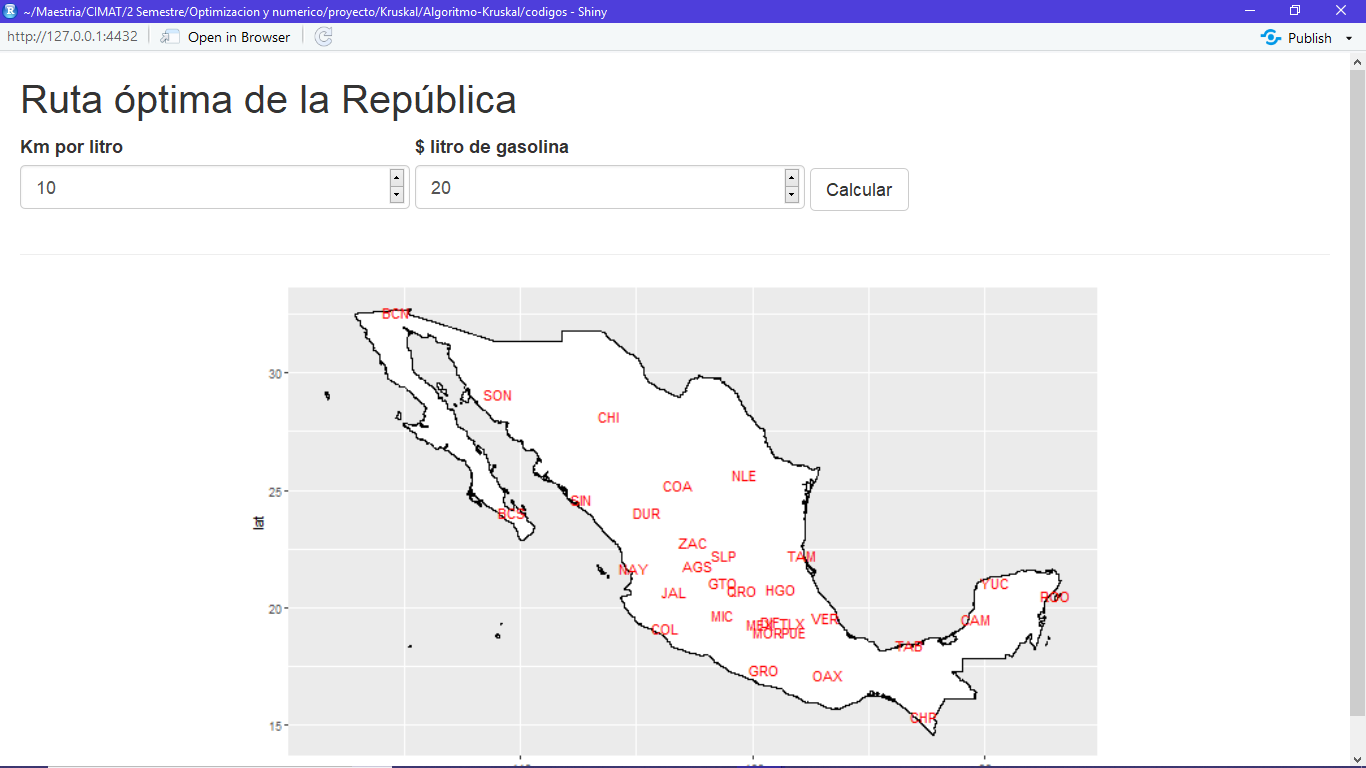
\includegraphics[scale=.45]{i2.png} 
\label{i2}
\caption{Aplicativo generado.}
\end{figure}

Con los valores por defecto se calcula el árbol de pesos mínimo, el cual se muestra en la figura 3, generando un costo de \$24,618\\

\begin{figure}
\centering
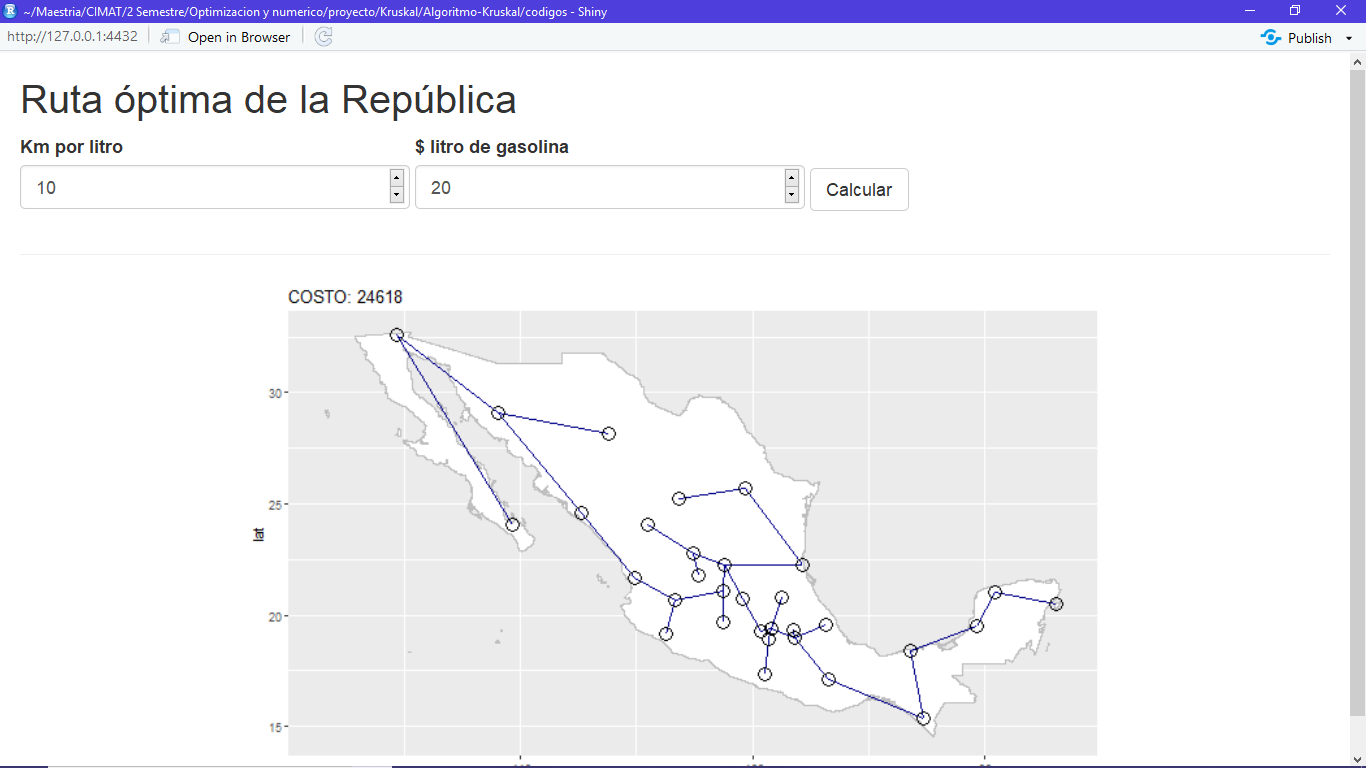
\includegraphics[scale=.45]{i3.png} 
\caption{Árbol con los parámetros por defecto}
\end{figure}

Además, se modifican los valores para visualizar como cambia la solución al variar los parámetros, en la figura 4 se aprecia como el costo total se modifica, así como la estructura del árbol. Para estos valores, el costo es \$18,080\\

\begin{figure}
\centering
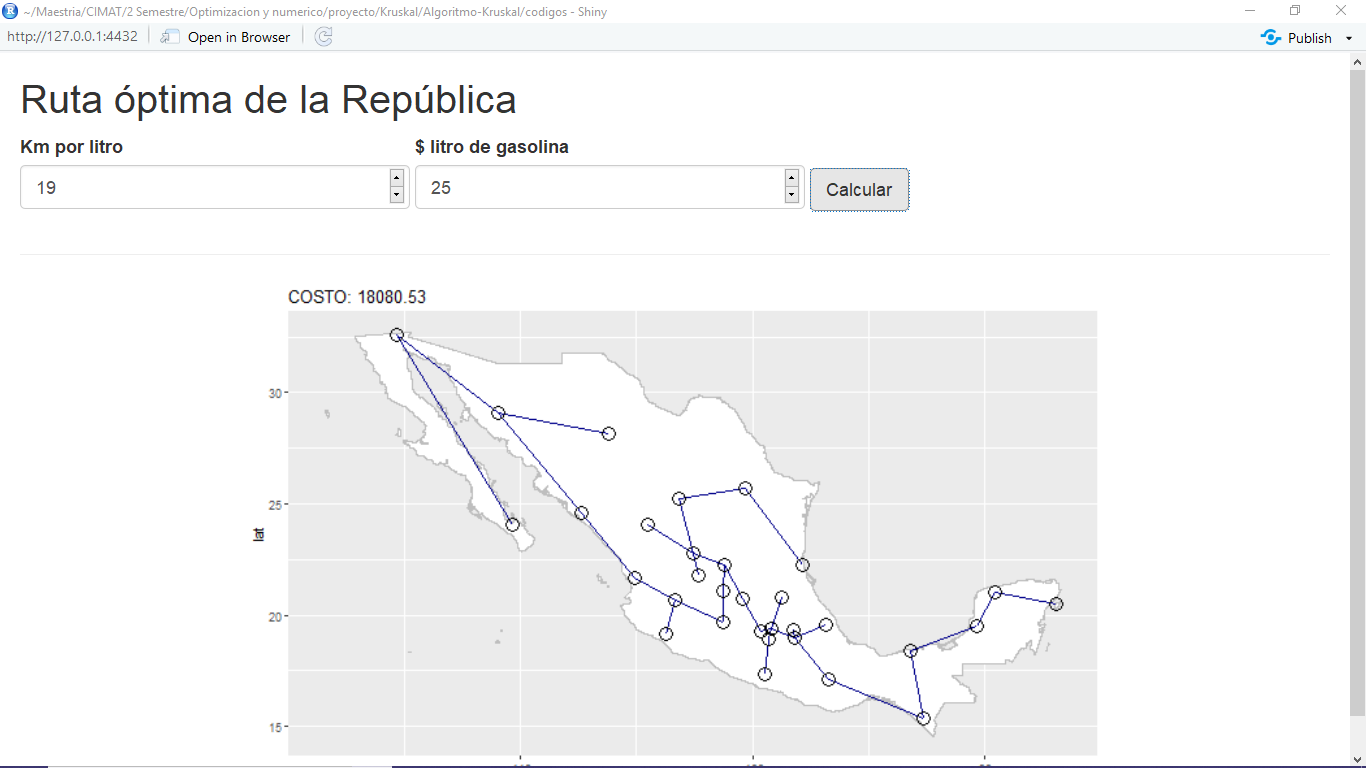
\includegraphics[scale=.45]{i4.png} 
\caption{Árbol considerando rendimiento de 19km/lt y costo de \$25 el lt de gasolina}
\end{figure}


\section{Trabajos futuros}
El trabajo que se presentó puede ser aplicado considerando más costos, por ejemplo, tiempo y desgaste del vehículo.\\

Además, se puede modificar para considerar solo las ciudades de interés para algún interés en específico.\\

También se puede buscar ligarlo a algún servidor en el cual se actualicen los precios de combustibles y casetas en la República Mexicana.\\

Así como buscar alguna API, para extraer la información de distancias entre capitales de manera automática.
\end{document}